%! Author = petter
%! Date = 04.01.2021

\chapter{Implementation}\label{ch:implementation}

In this chapter we are going to look at the implementation of PTS.

\section{Compiler Architecture}\label{sec:architecture}

\begin{figure}
   \centering
   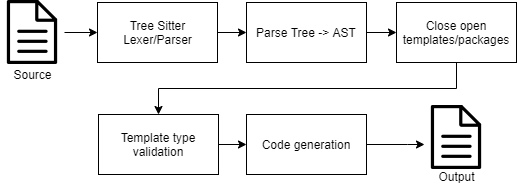
\includegraphics[scale=.75]{images/Compiler overview.png}
   \caption{Overview of the compiler}
   \label{fig:compiler-overview}
\end{figure}

\section{Lexer and Parser}\label{sec:lexer-and-parser}


\subsection{Parser Generator}\label{subsec:parser-generator}

There are a lot of parser generators out there, but there is no one-size-fits-all solution.
In order to navigate through the sea of options we need to set some requirements in functionality, so that we can more easily find the right tool for the task.

As we talked about in section~\vref{sec:what-do-we-need}, we set ourselves the goal to find an approach that would allow us to create an implementation that was loosely coupled with TypeScript.
TypeScript is a large language that is constantly updated, and is getting new features fairly often.
Because of this one of the requirements for our choice of parser generator is the possibility for extending grammars.
This is important because we want to keep our grammar loosely coupled with the TypeScript grammar, and don't want to be forced to rewrite the entire TypeScript grammar, as well as keeping it up-to-date.

We will be working with the TypeScript API, which only has a runtime library in JavaScript/TypeScript.
Therefore, another desired attribute is a runtime library in TypeScript.
This is not as essential as the requirement above, as we can get around using the TypeScript API and instead use the TypeScript CLI, or create a CLI in the language of the parser generator tools runtime library.


\subsubsection{ANTLR4}\label{subsubsec:antlr}

ANTLR, ANother Tool for Language Recognition, is a very powerful and versatile tool, used by many, such as Twitter for query parsing in their search engine\cite{Terence2012}.

ANTLR supports extending grammars, or more specifically importing them.
Importing a grammar works much like a "smart include".
It will include all rules that are not already defined in the grammar.
Through this you can extend a grammar with new rules or replacing them.
It does not however support extending rules, as in referencing the imported rule while overriding\cite{Terence2012}.
This isn't a major issue however as you could easily rewrite the rule with the additions.

The only supported runtime library in ANTLR is in Java.
This does not mean that you won't be able to use it in any other language, as you could simply invoke the runtime library through command line, however it is worth keeping in mind.

Overall ANTLR seems like a good option for our project, but the lack of a runtime library in TypeScript is a hurdle we would rather get a round if we can.

\subsubsection{Bison}\label{subsubsec:bison}

Bison is a general-purpose parser generator.
It is one of many successors to Yacc, and is upwards compatible with Yacc\cite{bison}.

Bison does not support extending grammars.
The tool works on a single grammar file and produces a C/C++ program.
There is a possibility to include files, like with any other C/C++ program, in the grammar files prologue, however this will not allow us to include another grammar, as it only inserts the prologue into the generated parser.
In order to extend a grammar we would have to change the produced parser to include some extra rules.
Although this could possibly be automated by a script, it seems too hacky of a solution to consider.

On top of this Bison does not have a runtime library in JavaScript/TypeScript.
There does exist some ports/clones of Bison for JavaScript, such as \href{http://zaa.ch/jison/}{Jison} and \href{http://canna71.github.io/Jacob/}{Jacob}, however to my knowledge these also lack the functionality of extending grammars.

\subsubsection{Tree-sitter}\label{subsubsec:tree-sitter}

\href{https://tree-sitter.github.io/tree-sitter/}{Tree-sitter} is a fairly new parser generator tool, compared to the others in this list.
It aims to be general, fast, robust and dependency-free\cite{tree-sitter}.
The tool has been garnering a lot of traction the last couple of years, and is being used by Github, VS Code and Atom to name a few.
It has mainly been used in language servers and syntax highlighting, however it should still work fine for our compiler since it does produce a parse tree.

Although it isn't a documented feature, Tree-sitter does allow for extending grammars.
Extending a grammar works much like in ANTLR, where you get almost a superclass relation to the grammar.
One difference from ANTLR though is that it does allow for referencing the grammar we are extending during rule overriding.
This makes it easier and more robust to extend rules than in ANTLR.

Tree-sitter also has a runtime library for TypeScript, which makes it easier for us to use it in our implementation than the previous candidates.

Another cherry on top is that Tree-sitter is becoming one of the mainstream ways of syntax highlighting in modern editors and IDEs, which means that we could utilize the same grammar to get syntax highlighting for our language.

All this makes Tree-sitter stand out as the best candidate for our project.

\subsubsection{Implementing Our Grammar in Tree-sitter}

Tree-sitter uses the term rule instead of production, and I will therefore also refer to productions as rules here.

Extending a grammar in Tree-sitter works much like extending a class in an object-oriented language.
A "sub grammar" inherits all the rules from the "super grammar", so an empty ruleset would effectively work the same as the super grammar.
Just like most object-oriented languages have access to the super class, we also have access to the super grammar in Tree-sitter.
All of this enables us to add, override, and extend rules in an existing grammar, all while staying loosely coupled with the super grammar.
By extending the grammar, and not forking it, we are able to simply update our dependency on the TypeScript grammar, minimizing the possibility for conflicts.

As mentioned, Tree-sitter allows for referencing the super grammar during rule overriding, effectively making it possible to combine the old rule and the new.
A good example of overriding and combining rules can be found in the grammar of PTS, see listing~\vref{lst:overriding-combining-rule}, where we override the \codeword{\_declaration} rule from the TypeScript grammar, to include the possibility for package and template declarations.

\begin{code}{javascript}{Snippet from the PTS grammar, where we override the \codeword{\_declaration} rule from the TypeScript grammar, and adding two additional declarations.}{lst:overriding-combining-rule}
    _declaration: ($, previous) =>
        choice(
            previous,
            $.template_declaration,
            $.package_declaration
        )
\end{code}




\section{Notes on Performance}\label{sec:notes-on-performance}

Very slow compiler/PP because of the chosen implementation, with tree traverser for every step.


\section{Testing}\label{sec:testing}

\subsection{Lexer and Parser}\label{subsec:testing-lexer-and-parser}

Tree-sitter tests are simple \codeword{.txt} files split up into three sections, the name of the test, the code that should be parsed, and the expected parse tree in S-expressions\cite{sexprs}.

\begin{code}{typescript}{Example of tree-sitter grammar test}{lst:tree-sitter-grammar-test}
    ===========================
    Closed template declaration
    ===========================

    template T {
        class A {
            i = 0;
        }
    }

    ---
    (program
        (template_declaration
            name: (identifier)
            body: (package_template_body
                    (class_declaration
                        name: (type_identifier)
                        body: (class_body
                            (public_field_definition
                                name: (property_identifier)
                                value: (number)))))))

\end{code}

\subsection{Transpiler}\label{subsec:testing-transpiler}

Started with jest, and used some time to get it to work with typescript files, however had to switch because jest doesn't handle native libraries (tree-sitter) too well.
It \codeword{require}s the same native library several times, making the wrapping around the native program to break.